\section*{Assignment 7 Q3}
Find all solutions to the system:
\spl{
    2x&\equiv4(\bmod\ 5)\\
    3x&\equiv5(\bmod\ 7)\\
    7x&\equiv1(\bmod\ 13)
}

$\blacktriangleright$

Since
\spl{
    3\cdot2&\equiv1(\bmod\ 5)\\
    5\cdot3&\equiv1(\bmod\ 7)\\
    2\cdot7&\equiv1(\bmod\ 13)
}
then equivalently, we rewrite the system as
\spl{
    x&\equiv2(\bmod\ 5)\\
    x&\equiv4(\bmod\ 7)\\
    x&\equiv4(\bmod\ 13)\\
}
Since $m_1=5, m_2=7, m_3=13$ are pairwise relatively prime, then $[M_k]_{m_k}\in(\mathbb{Z}/m_k\mathbb{Z})^*$. Now $m=5\cdot7\cdot13=455$ and consider $$M_1=\frac{455}{5}=91,M_2=\frac{455}{7}=65,M_3=\frac{455}{13}=35$$
Note that $y_1=1$, $y_2=4$, $y_3=3$, then $$x=\sum_{k=1}^na_kM_ky_k=2\cdot91\cdot1+4\cdot65\cdot4+4\cdot35\cdot3=1642=277(\bmod\ 455)$$
Due to the uniqueness of solutions $(\bmod\ 455)$, all the solutions to this system are $$x=455k+277,\quad\forall k\in\mathbb{Z}$$

$\bigstar\bigstar\bigstar$\textbf{Get familiar with the procedure! Speed up your calculation!}

\section*{Assignment 8 Q1}
Prove that if ($a_n$) is a sequence that satisfies a linear homogeneous recurrence relation of degree 2 whose characteristic polynomial has only one real root $\alpha$, then there exists $q_1, q_2 \in\mathbb{R}$ such that for all $n \in \mathbb{N}$,
$$a_n=q_1\alpha^n+q_2n\alpha^n$$
$\blacktriangleright$ \begin{proof}
    Suppose that the characteristic equation of $a_n$ is $(\lambda-\alpha)^2=0$, then we have a linear homogeneous recurrence relation $$a_n=2\alpha a_{n-1}-\alpha^2a_{n-2},\quad n\geq2$$ with $a_0=u$ and $a_1=v$.
    
    Now we only consider that $\alpha\neq0$. Otherwise, $0^0$ does not make sense. Then we prove that there exists $q_1=u$ and $q_2=\frac{v-u\alpha}{\alpha}$ such that for all $n\in\mathbb{N}$, $$a_n=u\alpha^n+\frac{v-u\alpha}{\alpha}n\alpha^n$$

    First, it's easy to see that $a_0=u\alpha^0+0=u$ and $a_1=u\alpha+\frac{v}{\alpha}\alpha-u\alpha=v$.

    For $n\geq2$,
    \spl{
        \textbf{LHS}&=a_n=q_1\alpha^n+q_2 n\alpha^n\\
        \textbf{RHS}&=2\alpha a_{n-1}-\alpha^2a_{n-2}\\
        &=2\alpha(q_1\alpha^{n-1}+q_2 (n-1)\alpha^{n-1})-\alpha^2(q_1\alpha^{n-2}+q_2 (n-2)\alpha^{n-2})\\
        &=(2q_1-q_1)\alpha^n+q_2(2n-2-n+2)\alpha^n\\
        &=q_1\alpha^n+q_2 n\alpha^n\\
        &=\textbf{LHS}
    }
\end{proof}

$\bigstar\bigstar\bigstar$\textbf{To prove the existence? Just find it!}

\section*{Assignment 8 Q4}
Find an expression for the terms of the sequence ($a_n$) that satisfy $$a_n = 7a_{n-1}-16a_{n-2} + 12a_{n-3} + n4^n$$
with $a_0 = −3$, $a_1 = 2$, $a_2 = 5$.

$\blacktriangleright$

The characteristic equation is
\spl{
    \lambda^3-7\lambda^2+16\lambda-12&=0\\
    (\lambda-2)^2(\lambda-3)&=0
}

Hence the homogeneous part of $(a_n)$ has the form $$a_n=q_12^n+q_2n2^n+q_33^n$$ Since $f^\prime(n)=n4^n$, then we guess the particular solution is $$p(n)=c_0n4^n+c_14^n$$ This requires
\spl{
    c_0n4^n+c_14^n&=7(c_0(n-1)4^{n-1}+c_14^{n-1})-16(c_0(n-2)4^{n-2}+c_14^{n-2})\\
    &+12(c_0(n-3)4^{n-3}+c_14^{n-3})+n4^n\\
    &=(16+15c_0)n4^{n-2}+(15c_1-5c_0)4^{n-2}
}

\begin{equation*}
    \begin{cases}
        c_0=1+\frac{15}{16}c_0\\
        c_1=\frac{15}{16}c_1-\frac{5}{16}c_0\\
    \end{cases}
    \Rightarrow
    \begin{cases}
        c_0=16\\
        c_1=-80\\
    \end{cases}
\end{equation*}

This means that $(a_n)$ has the form $$a_n=q_12^n+q_2n2^n+q_33^n+16n4^n-80\cdot4^n$$
Thus
\begin{equation*}
    \left(\begin{array}{ccccc}
        1&0&1&\vline&-3-(-80)\\
        2&2&3&\vline&2-(-256)\\
        4&8&9&\vline&5-(-768)\\
    \end{array}\right)
    \sim
    \left(\begin{array}{ccccc}
        1&0&0&\vline&28\\
        0&1&0&\vline&\frac{55}{2}\\
        0&0&1&\vline&49
    \end{array}\right)
\end{equation*}

Thus $$a_n=28\cdot2^n+\frac{55}{2}n2^n+49\cdot3^n+16n4^n-80\cdot4^n$$

$\bigstar\bigstar\bigstar$\textbf{For particular solutions, start from the multiplicity of $s$}

\section*{Assignment 8 Q5}
For all $n\in\mathbb{N}\backslash\{0\}$, let
$$a_n=\sum_{i=1}^ni^4$$
By finding a recurrence relation that ($a_n$) satisfies and solving that recurrence relation, find an expression for the terms of the sequence ($a_n$).

$\blacktriangleright$ $$a_n=a_{n-1}+n^4,\quad a_1=1$$
Since $\lambda=1$, then the homogeneous part of $(a_n)$ is $q_11^n=q_1$.
On the other hand, since $n^4=n^4\times1^n$, the particular part is $$p(n)=c_5n^5+c_4n^4+c_3n^3+c_2n^2+c_1n$$ Thus
\spl{
    &c_5n^5+c_4n^4+c_3n^3+c_2n^2+c_1n\\
    =&c_5(n-1)^5+c_4(n-1)^4+c_3(n-1)^3+c_2(n-1)^2+c_1(n-1)+c_0+n^4\\
    =&c_5n^5+(c_4-5c_5+1)n^4+(c_3-4c_4+10c_5)n^3+(c_2-3c_3+6c_4-10c_5)n^2\\
    +&(c_1-2c_2+3c_3-4c_4+5c_5)n-c_1+c_2-c_3+c_4-c_5
}

\begin{equation*}
    \begin{cases}
        c_4=c_4-5c_5+1\\
        c_3=c_3-4c_4+10c_5\\
        c_2=c_2-3c_3+5c_4-10c_5\\
        c_1=c_1-2c_2+3c_3-4c_4+5c_5\\
        0=-c_1+c_2-c_3+c_4-c_5
    \end{cases}
    \Rightarrow
    \begin{cases}
        c_5=\frac{1}{5}\\
        c_4=\frac{1}{2}\\
        c_3=\frac{1}{3}\\
        c_2=0\\
        c_1=-\frac{1}{30}\\
    \end{cases}
\end{equation*}

This means that $(a_n)$ has the form $$a_n=q_1+\frac{1}{5}n^5+\frac{1}{2}n^4+\frac{1}{3}n^3-\frac{1}{30}n$$
Since $a_1=1$, then $q_1=0$。
Thus $$a_n=\frac{1}{5}n^5+\frac{1}{2}n^4+\frac{1}{3}n^3-\frac{1}{30}n$$

$\bigstar\bigstar\bigstar$ \textbf{When $f^\prime(n)$ is a polynomial, imagine $1^n$}

\section*{Assignment 8 Q6}
Q6. Solve the simultaneous recurrence relations
\begin{equation*}
    \begin{cases}
        a_n=3a_{n-1}+2b_{n-1}\\
        b_n=a_{n-1}+2b_{n-1}
    \end{cases}
\end{equation*}
with $a_0 = 1$ and $b_0 = 2$.

$\blacktriangleright$

We multiply the second equation by $3$
\begin{equation*}
    \begin{cases}
        a_n=3a_{n-1}+2b_{n-1}\\
        3b_n=3a_{n-1}+6b_{n-1}
    \end{cases}
\end{equation*}
Then we subtract the difference back to the second equation
\spl{
    a_n&=3b_n-4b_{n-1}\\
    b_n&=(3b_{n-1}-4b_{n-2})+2b_{n-1}\\
    &=5b_{n-1}-4b_{n-2}
}
Since $a_0=1$ and $b_0=2$, then $b_1=a_0+2b_0=5$.

Thus $b_n=1+4^n$.

Similarly, $a_n=5a_{n-1}-4a_{n-2}$ with $a_0=1$ and $a_1=7$. Thus $a_n=-1+2\cdot4^n$

Therefore,
\spl{
    a_n&=-1+2\cdot4^n\\
    b_n&=1+4^n
}

$\bigstar\bigstar\bigstar$ \textbf{Substitution!}
\section*{Assignment 8 Q11}
Prove that if $n\in\mathbb{N}$ with $n\geq4$, then there exists a 3-regular graph of order $n$ if
and only if $n$ is even.

$\blacktriangleright$ \begin{proof}
$\Rightarrow$: Since it's a 3-regular graph, we obtain the total edge number $$|E|=\frac{3|V|}{2}=\frac{3n}{2}$$ Since $|E|$ has to be an integer, then $n$ is even.

$\Leftarrow$: Since $n$ is even, then we apply induction.

Let $P(n)$ be that for all $n\geq4$ and $n$ is even, there exists a 3-regular graph.

$P(4)$ holds since $K_4$.

Assume $P(k)$ holds. For $n=k+2$, here gives the procedure to get a 3-regular graph with order $k+2$ (denoted as $G_{k+2}$) from a 3-regular graph with order $k$ (denoted as $G_{k}$).
\begin{enumerate}
    \item Consider a pair of new vertices with new edge $(v_{k}, v_{k+1})$
    \item Break an arbitrary edge $(v_0, v_1)$ from $G_{k}$. Build edges $(v_0, v_{k})$ and $(v_1, v_{k})$
    \item Break an arbitrary edge $(v_2, v_3)$ from $G_{k}$. Build edges $(v_2, v_{k})$ and $(v_3, v_{k})$
\end{enumerate}
The degree of every vertex is 3. $P(k+2)$ holds.

Thus $P(n)$ holds for $n\geq4$ and $n$ is even.
\end{proof}

\section*{Assignment 8 Q13}
Let $G$ be a graph of order $10$ and size $15$.
\begin{enumerate}
    \item Is it the case that $\Delta(G) \geq 3$?
    
    $\blacktriangleright$ \begin{proof}
    Suppose $\Delta(G)\leq2$, then $$|E|=15=\frac{\sum d_G(v)}{2}\leq\frac{|V|\times \Delta(G)}{2}\leq\frac{|V|\times2}{2}=|V|=10$$
    which leads to contradiction.
    
    Hence $\Delta(G)\geq3$ holds.
    \end{proof}
    \item Is it the case that $\delta(G) \geq 2$?
    
    $\blacktriangleright$\begin{proof}
    Find a counterexample 
    \begin{figure}[h]
        \centering
        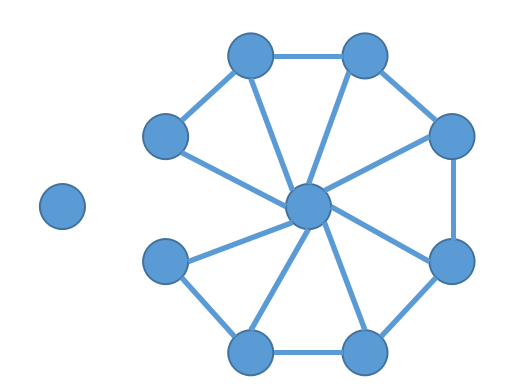
\includegraphics[width=0.55\textwidth]{example.png}
        \caption{order$=10$, size$=15$}
        \label{fig:example}
    \end{figure}
    where $\delta(G)=0$
    \end{proof}
\end{enumerate}
$\bigstar\bigstar\bigstar$ \textbf{Understand $\delta(G)$ and $\Delta(G)$! Use it in inequalities!}
